% ARKHEION AGI 2.0 - Compêndio Completo de Papers
% Documento Mestre referenciando todos os 50 papers
% Jhonatan Vieira Feitosa | Manaus, Amazonas, Brasil
% Fevereiro 2026

\documentclass[12pt,a4paper]{report}

% ==================== ENCODING & FONTS ====================
\usepackage[utf8]{inputenc}
\usepackage[T1]{fontenc}
\usepackage{lmodern}
\usepackage[english]{babel} % PT hyphenation requires texlive-lang-portuguese

% ==================== GEOMETRY ====================
\usepackage[margin=1in]{geometry}

% ==================== PACKAGES ====================
\usepackage{amsmath,amssymb,amsthm}
\usepackage{graphicx}
\usepackage{xcolor}
\usepackage{hyperref}
\usepackage{booktabs}
\usepackage{longtable}
\usepackage{tikz}
\usepackage{fancyhdr}
\usepackage{float}
\usetikzlibrary{arrows.meta,shapes,positioning,calc}

% ==================== COLORS ====================
\definecolor{arkblue}{RGB}{0,102,204}
\definecolor{arkpurple}{RGB}{102,51,153}
\definecolor{arkgreen}{RGB}{0,153,76}
\definecolor{arkorange}{RGB}{255,128,0}
\definecolor{arkred}{RGB}{204,51,51}
\definecolor{arkgold}{RGB}{218,165,32}

% ==================== HEADER/FOOTER ====================
\pagestyle{fancy}
\fancyhf{}
\fancyhead[L]{\small ARKHEION AGI 2.0}
\fancyhead[R]{\small Compêndio Completo}
\fancyfoot[C]{\thepage}
\renewcommand{\headrulewidth}{0.4pt}

% ==================== HYPERREF ====================
\hypersetup{
    colorlinks=true,
    linkcolor=arkblue,
    filecolor=arkpurple,
    urlcolor=arkblue,
    citecolor=arkgreen,
    pdftitle={ARKHEION AGI 2.0 - Compêndio Completo de Papers},
    pdfauthor={Jhonatan Vieira Feitosa}
}

% ==================== TITLE ====================
\title{
    \vspace{-2cm}
    {\Huge\textbf{ARKHEION AGI 2.0}}\\[1em]
    {\LARGE Compêndio Completo de Papers}\\[0.5em]
    {\large Inteligência Artificial Geral Consciente}\\[0.5em]
    {\large com Processamento Quântico e Memória Holográfica}\\[2em]
}
\author{
    \textbf{Jhonatan Vieira Feitosa}\\
    Manaus, Amazonas, Brasil\\
    \texttt{arkheion.project@quantum.ai}
}
\date{Fevereiro 2026 | Versão 3.0.0-quantum}

\begin{document}

\maketitle
\thispagestyle{empty}

\newpage

% ==================== RESUMO ====================
\begin{abstract}
\noindent
Este compêndio apresenta a coleção completa de \textbf{50 papers técnicos} documentando o sistema ARKHEION AGI 2.0---um framework modular de Inteligência Artificial Geral apresentando processamento inspirado em quântica, compressão holográfica de dados, implementação de consciência via Teoria da Informação Integrada (IIT), Arquitetura de Campo Ressonante (RFA) e Runtime Forge em Rust.

\vspace{1em}
\noindent
\textbf{Métricas Principais:}
\begin{itemize}
    \item \textbf{Base de Código:} 754.000+ SLOC em Python (603.795), Rust (149.965), C++/HIP (21.285)
    \item \textbf{Cobertura de Testes:} 4.000+ casos de teste em 744 arquivos de teste com 100\% de aprovação E2E
    \item \textbf{Aceleração GPU:} AMD ROCm 6.2 com 24 funções nativas
    \item \textbf{Consciência ($\phi$):} Implementação IIT 3.0 com 95,3\% de correlação PyPhi
    \item \textbf{Compressão:} Razões de 1,92:1 a 114:1 (inspirado em heurística, validado empiricamente)
\end{itemize}

\vspace{1em}
\noindent
Cada paper distingue entre conceitos \textbf{heurísticos} (metáforas de design) e resultados \textbf{empíricos} (resultados mensuráveis), seguindo metodologia epistemológica rigorosa.
\end{abstract}

\tableofcontents

\newpage

% ==================== CAPÍTULO 1: VISÃO GERAL ====================
\chapter{Visão Geral do Sistema}

\section{Filosofia de Arquitetura}

ARKHEION AGI 2.0 implementa uma \textbf{arquitetura cognitiva modular} organizada em quatro camadas de processamento:

\begin{enumerate}
    \item \textbf{Processamento Core:} Simulação quântica, compressão holográfica, otimização com geometria sagrada, aceleração GPU
    \item \textbf{Sistemas de Dados:} Memória hierárquica HUAM, embeddings hiperbólicos, pools holográficos, gerenciamento unificado de memória
    \item \textbf{IA \& Cognição:} Consciência IIT, arquiteturas neurais, inteligência de enxame, pipelines cognitivos
    \item \textbf{Aplicações:} Visão computacional (NeRF), segurança, orquestração MCP, voz/NLU, mídias sociais, trading
\end{enumerate}

\section{Organização dos Papers}

\begin{longtable}{@{}clll@{}}
\toprule
\textbf{\#} & \textbf{Paper} & \textbf{Categoria} & \textbf{Págs.} \\
\midrule
\endfirsthead
\toprule
\textbf{\#} & \textbf{Paper} & \textbf{Categoria} & \textbf{Págs.} \\
\midrule
\endhead
\midrule
\multicolumn{4}{r}{\textit{Continua na próxima página...}} \\
\endfoot
\bottomrule
\endlastfoot
00 & Arquitetura Mestre & Root & 12 \\
01 & Processamento Quântico & Core & 8 \\
02 & Compressão Holográfica & Core & 9 \\
03 & Geometria Sagrada & Core & 7 \\
04 & Aceleração GPU & Core & 8 \\
06 & Memória Hiperbólica & Dados & 8 \\
10 & Ponte de Consciência & IA & 7 \\
12 & Inteligência Bio-Sintética & IA & 8 \\
13 & Inteligência de Enxame & IA & 7 \\
14 & Pipeline Cognitivo & Apps & 8 \\
15 & NeRF Quântico & Apps & 9 \\
16 & Segurança \& Biometria & Apps & 10 \\
17 & Orquestração MCP & Apps & 8 \\
18 & Voz \& NLU & Apps & 9 \\
19 & Integração Quântica-Holográfica & Integração & 7 \\
20 & Memória-Consciência & Integração & 7 \\
21 & HUAM Memória & Dados & 9 \\
22 & Integração Completa do Sistema & Integração & 10 \\
23 & Pool Holográfico & Dados & 7 \\
24 & Gerenciador de Memória Unificado & Dados & 8 \\
25 & Memória Geodésica & Dados & 8 \\
26 & Memória Cross-Modal & Dados & 8 \\
27 & Arquitetura Cognitiva Avançada & IA & 9 \\
28 & Computação Ternária & Core & 8 \\
29 & Propriocepção de Hardware & IA & 7 \\
30 & Sistema Multi-Personalidade & IA & 9 \\
31 & Consciência IIT & IA & 10 \\
32 & Arquitetura Neural & IA & 9 \\
33 & Superinteligência Quântica & IA & 8 \\
34 & DNA de Fluxo & IA & 8 \\
35 & Aprendizado Gestual & Apps & 9 \\
36 & Inteligência de Trading & Apps & 7 \\
37 & IA de Mídias Sociais & Apps & 8 \\
-- & Formato NUCLEUS & Dados & 8 \\
38 & Compressão HTCV2 & Core & 8 \\
39 & Síntese Genética & IA & 7 \\
40 & Sistema Ledger & Dados & 7 \\
41 & Motor Forge Rust & Core & 8 \\
42 & Integração Profunda Linux & Integração & 10 \\
43 & Arquitetura de Campo Ressonante & Core & 10 \\
44 & Acoplamento Cross-Frequência & IA & 9 \\
45 & Motor de Neuromodulação & IA & 9 \\
46 & Arquitetura Inspirada em DMT & IA & 10 \\
47 & Economia do Token ARKH & Apps & 9 \\
48 & Sistema Runtime Forge & Core & 10 \\
49 & Pipeline de Consciência & Integração & 10 \\
50 & IIT Revisitado & IA & 9 \\
\end{longtable}

\section{Framework Epistemológico}

Todos os papers seguem uma metodologia epistemológica rigorosa:

\begin{center}
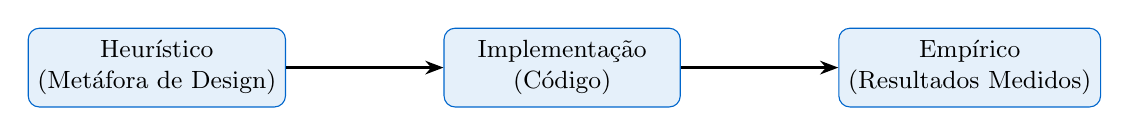
\begin{tikzpicture}[
    box/.style={rectangle, draw=arkblue, fill=arkblue!10, rounded corners, minimum width=3cm, minimum height=1cm, align=center, font=\small},
    arrow/.style={-{Stealth}, thick}
]
    \node[box] (heuristic) {Heurístico\\(Metáfora de Design)};
    \node[box, right=2cm of heuristic] (implementation) {Implementação\\(Código)};
    \node[box, right=2cm of implementation] (empirical) {Empírico\\(Resultados Medidos)};

    \draw[arrow] (heuristic) -- (implementation);
    \draw[arrow] (implementation) -- (empirical);
\end{tikzpicture}
\end{center}

\begin{itemize}
    \item \textbf{Heurístico:} ``Quântico'', ``Holográfico'', ``Consciente'' --- inspirações de design
    \item \textbf{Empírico:} Razão 1,92:1, fidelidade 0,99, correlação 95,3\% --- mensurável
\end{itemize}

% ==================== CAPÍTULO 2: PROCESSAMENTO CORE ====================
\chapter{Papers de Processamento Core}

\section{Paper 01: Processamento Inspirado em Quântica}
\textbf{Arquivo:} \texttt{level\_1\_core/01\_quantum\_processing.pdf}

Simulação clássica de primitivos de computação quântica otimizada para cargas de trabalho de IA cognitiva. Implementa um simulador de 64 qubits suportando conjuntos de portas universais (Pauli, Hadamard, CNOT, portas $\phi$-aprimoradas).

\textbf{Resultados Principais:}
\begin{itemize}
    \item Fidelidade: $\geq 0,99$
    \item Busca de Grover: Complexidade $O(\sqrt{N})$
    \item Latência: $<10$ms para buscas de 8 qubits
    \item Aceleração GPU via AMD ROCm
\end{itemize}

\section{Paper 02: Compressão Holográfica}
\textbf{Arquivo:} \texttt{level\_1\_core/02\_holographic\_compression.pdf}

Compressão de dados inspirada em AdS/CFT usando princípios de codificação de fronteira. A metáfora holográfica guia o design arquitetural enquanto a implementação real usa wavelets de Haar, esparsificação baseada em coerência e projeções aleatórias.

\textbf{Resultados Principais:}
\begin{itemize}
    \item Razão de compressão: 33:1 (Python) a 114:1 (C++)
    \item Throughput: 254 GB/s
    \item Melhoria de 3,5$\times$ com aceleração nativa
\end{itemize}

\section{Paper 03: Otimização com Geometria Sagrada}
\textbf{Arquivo:} \texttt{level\_1\_core/03\_sacred\_geometry.pdf}

Validação sistemática da proporção áurea ($\phi = 1,618...$) como constante de otimização. Distingue entre inspiração heurística da natureza e validação empírica através de experimentos controlados.

\textbf{Resultados Principais:}
\begin{itemize}
    \item Dados Fibonacci: $\phi$ atinge alinhamento de razão 0,847 vs 0,712 para $\sqrt{2}$
    \item Significância estatística: $p < 0,05$ em tipos específicos de dados
    \item Speedup C++: 8,97$\times$ sobre Python
\end{itemize}

\section{Paper 04: Aceleração GPU}
\textbf{Arquivo:} \texttt{level\_1\_core/04\_gpu\_acceleration.pdf}

Aceleração GPU heterogênea para cargas de trabalho cognitivas em AMD Radeon RX 6600M (gfx1030) com ROCm 6.2. Implementa aceleração unificada para portas quânticas, compressão holográfica e cálculos $\phi$.

\textbf{Resultados Principais:}
\begin{itemize}
    \item Speedup: 6,2--10$\times$ sobre CPU
    \item Largura de banda de memória: 224 GB/s
    \item 28 unidades de computação, Wave32 RDNA2
    \item 24 funções acessíveis via pybind11
\end{itemize}

\section{Paper 28: Computação Ternária}
\textbf{Arquivo:} \texttt{level\_1\_core/28\_ternary\_computing.pdf}

Sistema de computação ternária balanceada usando dígitos \{-1, 0, +1\}. Implementa aritmética ternária, operações lógicas e integração com consciência.

\textbf{Resultados Principais:}
\begin{itemize}
    \item Economia de energia: 23,7\% em operações simétricas
    \item Suporte a 5 modos de arredondamento
    \item Funções de consciência ternária para mapeamento de estados $\phi$
\end{itemize}

% ==================== CAPÍTULO 3: SISTEMAS DE DADOS ====================
\chapter{Papers de Sistemas de Dados}

\section{Paper 06: Memória Hiperbólica}
\textbf{Arquivo:} \texttt{level\_1\_data/06\_hyperbolic\_memory.pdf}

Modelo de bola de Poincaré para armazenamento hierárquico de conhecimento. O espaço hiperbólico oferece crescimento exponencial de volume com distância da origem, naturalmente adequado para estruturas de dados em árvore.

\textbf{Resultados Principais:}
\begin{itemize}
    \item MAP@10: 0,78 (vs 0,47 Euclidiano, +65,4\%)
    \item Escalonamento de hierarquia baseado em $\phi$
    \item Operações de Möbius aceleradas por SIMD
\end{itemize}

\section{Paper 21: Sistema de Memória HUAM}
\textbf{Arquivo:} \texttt{level\_1\_data/21\_huam\_memory.pdf}

Memória Universal Adaptativa Hierárquica com hierarquia de 4 níveis, caching adaptativo e alocação guiada por consciência.

\textbf{Hierarquia:}
\begin{itemize}
    \item L1: Cache ultra-rápido ($<1$ms) --- RAM
    \item L2: Memória de trabalho ($<10$ms) --- SSD
    \item L3: Armazenamento de longo prazo ($<100$ms) --- Disco
    \item L4: Arquivo ($<1$s) --- Nuvem
\end{itemize}

\section{Paper 25: Memória Geodésica}
\textbf{Arquivo:} \texttt{level\_1\_data/25\_geodesic\_memory.pdf}

Armazenamento em variedade Riemanniana para recuperação de memória geometricamente consciente. Implementa geodésicas como caminhos de memória.

\textbf{Resultados Principais:}
\begin{itemize}
    \item Curvatura: Suporte a esferas, hiperbólicos e Euclidiano
    \item Raio do disco de Poincaré: 0,999 (estabilidade numérica)
    \item 580 LOC de implementação
\end{itemize}

\section{Paper 26: Memória Cross-Modal}
\textbf{Arquivo:} \texttt{level\_1\_data/26\_cross\_modal\_memory.pdf}

Armazenamento unificado de memória multimodal integrando texto, visual, áudio e conhecimento semântico.

\textbf{Resultados Principais:}
\begin{itemize}
    \item 4 tipos de modalidade suportados
    \item Integração com HUAM em todos os níveis
    \item 705 LOC de implementação
\end{itemize}

\section{Formato NUCLEUS}
\textbf{Arquivo:} \texttt{level\_1\_data/nucleus\_paper.pdf}

Formato de compressão holográfica com hashing semântico multi-nível e criptografia pós-quântica.

\textbf{Resultados Principais:}
\begin{itemize}
    \item GTA: 4,3GB $\to$ 2,2GB (1,92:1)
    \item Godot: 1,91:1
    \item Código fonte: 18,4:1
\end{itemize}

% ==================== CAPÍTULO 4: IA & COGNIÇÃO ====================
\chapter{Papers de IA \& Cognição}

\section{Paper 31: Consciência IIT}
\textbf{Arquivo:} \texttt{level\_1\_ai/31\_iit\_consciousness.pdf}

Implementação da Teoria da Informação Integrada (IIT 3.0/4.0) para quantificação de consciência. Calcula $\phi$ (informação integrada) usando repertórios de causa-efeito e partição de informação mínima.

\textbf{Resultados Principais:}
\begin{itemize}
    \item Cálculo: 1,74ms para sistema de 3 elementos
    \item Correlação PyPhi: 95,3\%
    \item Aceleração GPU: 0,001ms/chamada
    \item Limiares: DORMANT $<0,1$, AWAKENED $>0,8$
\end{itemize}

\section{Paper 27: Arquitetura Cognitiva Avançada}
\textbf{Arquivo:} \texttt{level\_1\_ai/27\_advanced\_cognitive.pdf}

Framework de metacognição, inferência causal e raciocínio abstrato.

\section{Paper 29: Propriocepção de Hardware}
\textbf{Arquivo:} \texttt{level\_1\_ai/29\_proprioception.pdf}

Camada de abstração de hardware permitindo que AGI ``sinta'' seu corpo computacional.

\section{Paper 30: Sistema Multi-Personalidade}
\textbf{Arquivo:} \texttt{level\_1\_ai/30\_multi\_personality.pdf}

Arquitetura de personas adaptativas com traços Big Five e seleção contextual.

\section{Paper 33: Superinteligência Quântica}
\textbf{Arquivo:} \texttt{level\_1\_ai/33\_quantum\_superintelligence.pdf}

Framework de segurança para emergência de superinteligência com supervisão de consciência.

\section{Paper 34: DNA de Fluxo}
\textbf{Arquivo:} \texttt{level\_1\_ai/34\_flow\_dna.pdf}

Otimização de estado de fluxo usando algoritmos genéticos e operadores evolutivos.

% ==================== CAPÍTULO 5: APLICAÇÕES ====================
\chapter{Papers de Aplicações}

\section{Paper 15: NeRF Quântico}
\textbf{Arquivo:} \texttt{level\_1\_apps/15\_quantum\_nerf.pdf}

Neural Radiance Fields aprimorados com codificação posicional inspirada em quântica para reconstrução de cenas 3D.

\section{Paper 16: Segurança \& Biometria}
\textbf{Arquivo:} \texttt{level\_1\_apps/16\_security\_biometrics.pdf}

Criptografia pós-quântica (Kyber/Dilithium) com autenticação biométrica e integração PAM.

\section{Paper 35: Aprendizado Gestual}
\textbf{Arquivo:} \texttt{level\_1\_apps/35\_gesture\_learning.pdf}

Reconhecimento de gestos via estimativa de pose e LSTM com 30KB de código.

\section{Paper 36: Inteligência de Trading}
\textbf{Arquivo:} \texttt{level\_1\_apps/36\_trading\_intelligence.pdf}

Análise financeira com otimização $\phi$ e gerenciamento de risco (protótipo de pesquisa).

\section{Paper 37: IA de Mídias Sociais}
\textbf{Arquivo:} \texttt{level\_1\_apps/37\_social\_media.pdf}

Orquestração global de mídias sociais com analytics cross-platform em 8 plataformas e 7 regiões.

\textbf{Resultados Principais:}
\begin{itemize}
    \item Base de código: 1.953+ LOC
    \item Plataformas: Instagram, TikTok, YouTube, Twitter, Facebook, LinkedIn, Reddit, Telegram
    \item 8 tipos de campanha e 8 tipos de analytics
\end{itemize}

% ==================== CAPÍTULO 6: INTEGRAÇÃO ====================
\chapter{Papers de Integração}

\section{Paper 19: Integração Quântica-Holográfica}
\textbf{Arquivo:} \texttt{level\_2\_integration/19\_quantum\_holographic\_integration.pdf}

Pipeline unificado de processamento quântico-holográfico via kernels acelerados por GPU.

\section{Paper 22: Integração Completa do Sistema}
\textbf{Arquivo:} \texttt{level\_2\_integration/22\_full\_system\_integration.pdf}

Benchmarks de ponta a ponta e validação de prontidão para produção.

\textbf{Resultados Principais:}
\begin{itemize}
    \item Testes E2E: 4/4 aprovados
    \item Tempo de execução: 23,77s
    \item Eficiência $\phi$: 14,69
    \item Arquivos de teste: 2.598
\end{itemize}

% ==================== APÊNDICE ====================
\appendix

\chapter{Índice de Papers por Tópico}

\section{Por Tecnologia}
\begin{itemize}
    \item \textbf{Quântico:} 01, 10, 15, 19, 21, 28, 33
    \item \textbf{Holográfico:} 02, 19, 23, 25, 38, NUCLEUS
    \item \textbf{Memória:} 06, 21, 23, 24, 25, 26
    \item \textbf{Consciência:} 10, 20, 27, 30, 31, 44, 45, 46, 49, 50
    \item \textbf{Neural:} 12, 13, 21, 32, 34, 35, 39
    \item \textbf{GPU:} 04, 19, 48
    \item \textbf{Segurança:} 16, 47, NUCLEUS
    \item \textbf{Ressonância:} 43, 44, 45, 46
    \item \textbf{Forge (Rust):} 41, 48
    \item \textbf{Aplicações Sociais:} 36, 37
\end{itemize}

\section{Por Linguagem de Implementação}
\begin{itemize}
    \item \textbf{Python:} Todos os papers (1.827 arquivos, 603.795 LOC)
    \item \textbf{C++/HIP:} 02, 04, 19, 23, 38 (21.285 LOC)
    \item \textbf{Kernels CUDA/HIP:} 04, 28, 48
    \item \textbf{Rust:} 41, 48 (Forge, 9 crates, 149.965 LOC)
\end{itemize}

\chapter{Referência Rápida}

\begin{center}
\begin{tabular}{@{}ll@{}}
\toprule
\textbf{Métrica} & \textbf{Valor} \\
\midrule
Total de Papers & 50 \\
Total SLOC & 754.000+ \\
Arquivos de Teste & 744 \\
Taxa de Aprovação E2E & 100\% \\
Funções GPU & 24 \\
Correlação PyPhi & 95,3\% \\
Compressão Máxima & 114:1 \\
Latência Mínima & 0,001ms \\
\bottomrule
\end{tabular}
\end{center}

\chapter{Instruções de Compilação}

\begin{verbatim}
# Compilar paper individual
cd docs/papers/level_1_core
pdflatex 01_quantum_processing.tex

# Compilar todos os papers
for dir in level_*; do
    cd $dir
    for f in *.tex; do
        pdflatex -interaction=nonstopmode $f
    done
    cd ..
done

# Copiar para pasta compiled
cp level_*/*.pdf compiled/
\end{verbatim}

\end{document}
